
\documentclass[preprint,12pt]{elsarticle}

\usepackage[spanish]{babel}
\usepackage{amssymb}
\usepackage{graphicx}
\usepackage{lineno}
\usepackage[utf8]{inputenc}
\usepackage{url}
\usepackage{natbib} 
\usepackage{amsmath} 
\usepackage{amssymb} 

\begin{document}
	
	\begin{frontmatter}

		\title{\huge DevOps en Base de Datos}
		
		\author{Estrella Palacios, Katherine Lizbeth              	(2016056193))}
		\author{Gonzales Cave, Angel Gabriel              	(xxxxxxxxxx))} %%cambiar
		\author{Huichi Contreras, Franklin Carlos         	(2016054948))} %%cambiar
		\author{Huillca Umpiri, Willian Arturo             		(xxxxxxxxxx))} %%cambiar 
		\address{Tacna, Perú}
		
%% ABSTRACT --------------------------------------------------------------------------------------------------------------------

		\begin{abstract}
		
EDITAR

		\end{abstract}

%% ----------------------------------------------------------------------------------------------------------------------------------

	\end{frontmatter}

%% RESUMEN ---------------------------------------------------------------------------------------------------------------------

	\section{Resumen}

EDITAR

%% ----------------------------------------------------------------------------------------------------------------------------------


%% INTRODUCION ----------------------------------------------------------------------------------------------------------------

\section{Introducción} 

EDITAR

\begin{itemize}
\item A
\item B
\item C


\end{itemize}

%% ----------------------------------------------------------------------------------------------------------------------------------


%% MARCO TEÓRICO ------------------------------------------------------------------------------------------------------------

\section{Marco Teórico}

%% PRIMERA SUBSECCION 

\subsection {\textbf{A}}

\subsubsection{\textbf{A.1}}

EDITAR \cite{SQLne}  %% EJEMPLO DE COMO CITAR UNA REFERENCIA EN UN PÁRRAFO

\subsubsection{\textbf{A.2}}

EDITAR

\begin{figure}[htb]
	\begin{center}
		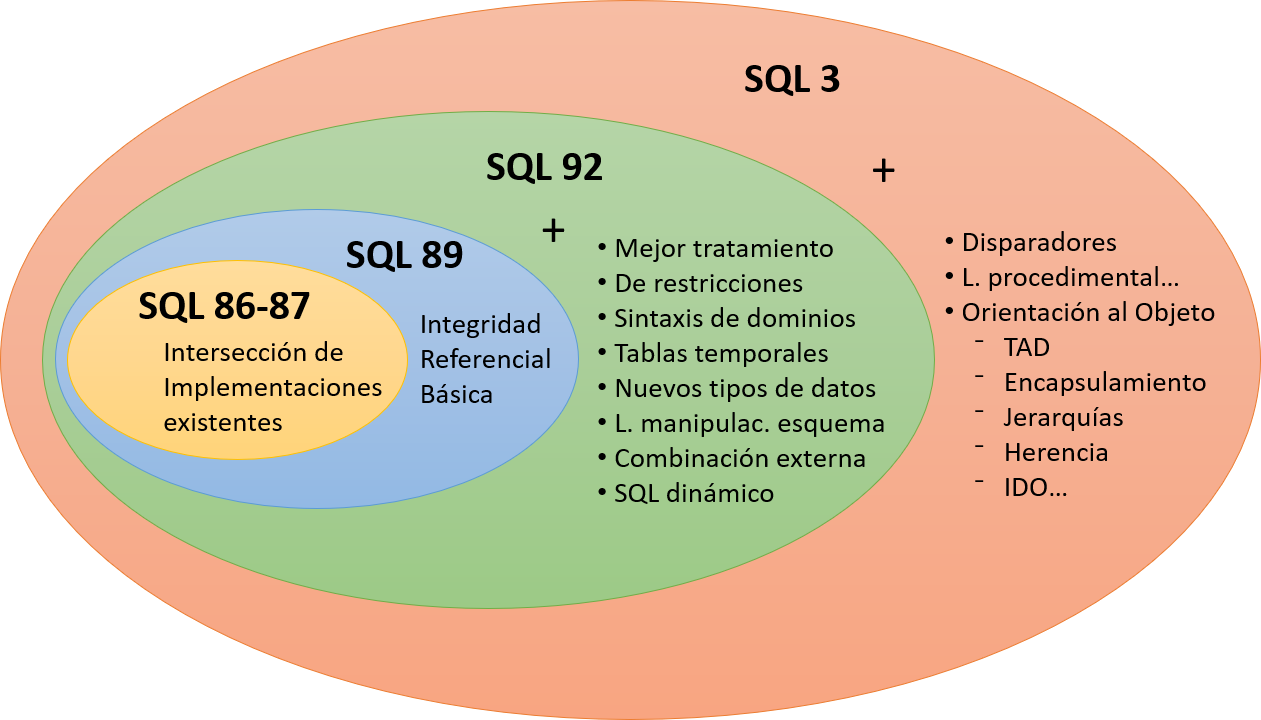
\includegraphics[width=10.5cm]{./IMAGENES/evolucion} %%EJEMPLO PARA INCLUIR IMAGEN
	\end{center}
\end{figure}


\subsubsection{\textbf{A.3}}

EDITAR

\begin{itemize}

\item x
\item y
\item z

\end{itemize}

%% SEGUNDA SUBSECCION

\subsection{\textbf{B}}

\subsubsection{\textbf{B.1}}

EDITAR

\subsubsection{\textbf{B.2}}	

EDITAR

\subsubsection{\textbf{B.3}}	

EDITAR


%% ----------------------------------------------------------------------------------------------------------------------------------


%% ANÁLISIS ( APLICACIÓN ) ---------------------------------------------------------------------------------------------------

\section{Análisis}

EDITAR

%% ----------------------------------------------------------------------------------------------------------------------------------


%% CONCLUSIONES ---------------------------------------------------------------------------------------------------------------

\section{Conclusiones}

\begin{itemize}

\item Conclusion 1 : \\ A

\item Conclusion 2 : \\ B

\item Conclusion 3 : \\ C

\end{itemize}

%% ----------------------------------------------------------------------------------------------------------------------------------

%%  REFERENCIAS BIBLIOGRÁFICAS ------------------------------------------------------------------------------------------
	
	\newpage
	
	\bibliographystyle{apalike} 	%ESTILO
	\bibliography{BIBLIOGRAFIA}	 
	
	
\end{document}
